\section{Apéndices}

\begin{frame}
    \begin{table}[]
        \centering
        \caption{Unidades básicas (UB) del SI}
        \label{tab:unidades_basicas_si}
        \resizebox{0.60\textwidth}{!}{
            \begin{tabular}{lll}
                \toprule
                Cantidad básica       & Nombre    & Símbolo     \\
                \midrule
                Longitud              & metro     & $\unit{m}$  \\
                Masa                  & kilogramo & $\unit{kg}$ \\
                Tiempo                & segundo   & $\unit{s}$  \\
                Corriente eléctrica   & ampere    & $\unit{A}$  \\
                Temperatura           & kelvin    & $\unit{K}$  \\
                Cantidad de sustancia & mol       & \unit{mol}  \\
                Intensidad luminosa   & candela   & $\unit{cd}$ \\
                \bottomrule
            \end{tabular}%
        }
    \end{table}
\end{frame}


\begin{frame}
    \begin{table}[]
        \centering
        \caption{Unidades SI derivadas}
        \label{tab:unidades_si_derivadas}
        \resizebox{1.00\textwidth}{!}{%
            \begin{tabular}{@{}lllll@{}}
                \toprule
                \textbf{Cantidad}         & \textbf{Nombre} & \textbf{Símbolo} & \textbf{Expresión en UB}              & \textbf{Expresión en otras unidades}  \\
                \midrule
                Ángulo plano              & radián          & rad              & $\unit{m/m}$                          & -                                     \\
                Frecuencia                & hertz           & Hz               & $\unit{s^{-1}}$                       & -                                     \\
                Fuerza                    & newton          & N                & $\unit{kg \cdot m/s^2}$               & $\unit{J/m}$                          \\
                Presión                   & pascal          & Pa               & $\unit{kg/m \cdot s^2}$               & $\unit{N/m^2}$                        \\
                Energía: trabajo          & joule           & J                & $\unit{kg \cdot m^2 / s^2}$           & $\unit{N \cdot m}$                    \\
                Potencia                  & watt            & W                & $\unit{kg \cdot m^2 / s^3}$           & $\unit{J/s}$                          \\
                Carga eléctrica           & coulomb         & C                & $\unit{A \cdot s}$                    & -                                     \\
                Potencial eléctrico (fem) & volt            & V                & $\unit{kg \cdot m^2 / A \cdot s^3}$   & $\unit{W/A, \quad J/C}$               \\
                Capacitancia              & farad           & F                & $\unit{A^2 \cdot s^4 / kg \cdot m^2}$ & $\unit{C/V}$                          \\
                Resistencia eléctrica     & ohm             & $\Omega$         & $\unit{kg \cdot m^2 / A^2 \cdot s^3}$ & $\unit{V/A}$                          \\
                Flujo magnético           & weber           & Wb               & $\unit{kg \cdot m^2 / A \cdot s^2}$   & $\unit{V \cdot s, \quad T \cdot m^2}$ \\
                Intensidad de c.m         & tesla           & T                & $\unit{kg/A \cdot s^2}$               & $\unit{Wb/m^2}$                       \\
                Inductancia               & henry           & H                & $\unit{kg \cdot m^2 / A^2 \cdot s^2}$ & $\unit{Wb/A}$                         \\
                \bottomrule
            \end{tabular}%
        }
    \end{table}
\end{frame}


\begin{frame}{}
    \begin{columns}
        \column{0.50\textwidth}
        \begin{table}
            \centering
            \caption{Prefijos para potencias de base 10}
            \resizebox{0.90\textwidth}{!}{%
                \begin{tabular}{@{}llc@{}}
                    \toprule
                    \textbf{Potencia de 10} & \textbf{Prefijo} & \textbf{Abreviatura} \\
                    \midrule
                    $10^{-24}$              & yocto-           & y                    \\
                    $10^{-21}$              & zepto-           & z                    \\
                    $10^{-18}$              & atto-            & a                    \\
                    $10^{-15}$              & femto-           & f                    \\
                    $10^{-12}$              & pico-            & p                    \\
                    $10^{-9}$               & nano-            & n                    \\
                    $10^{-6}$               & micro-           & $\mu$                \\
                    $10^{-3}$               & mili-            & m                    \\
                    $10^{-2}$               & centi-           & c                    \\
                    $10^{3}$                & kilo-            & k                    \\
                    $10^{6}$                & mega-            & M                    \\
                    $10^{9}$                & giga-            & G                    \\
                    $10^{12}$               & tera-            & T                    \\
                    $10^{15}$               & peta-            & P                    \\
                    $10^{18}$               & exa-             & E                    \\
                    $10^{21}$               & zetta-           & Z                    \\
                    $10^{24}$               & yotta-           & Y                    \\
                    \bottomrule
                \end{tabular}
            }
            \label{tab:Potencias_base_10}
        \end{table}

        \column{0.50\textwidth}
        \begin{table}[]
            \centering
            \caption{Símbolos matemáticos}
            \resizebox{0.95\textwidth}{!}{%
                \begin{tabular}{@{}ll@{}}
                    \toprule
                    \textbf{Símbolo} & \textbf{Significado}                 \\
                    \midrule
                    $=$              & es igual que                         \\
                    $\neq$           & no es igual que                      \\
                    $\equiv$         & se define como                       \\
                    $\propto$        & es proporcional a                    \\
                    $>$              & es mayor que                         \\
                    $<$              & es menor que                         \\
                    $\gg$            & es mucho mayor que                   \\
                    $\ll$            & es mucho menor que                   \\
                    $\approx$        & es aproximadamente igual que         \\
                    $\Delta x$       & cambio en $x$ o incertidumbre en $x$ \\
                    $\Sigma x_i$     & suma de todas las cantidades $x_i$   \\
                    $|x|$            & valor absoluto de $x$ siempre es +   \\
                    \bottomrule
                \end{tabular}%
            }
            \label{tab:my-table}
        \end{table}

    \end{columns}
\end{frame}

\begin{frame}
    \begin{table}
        \centering
        \caption{Alfabeto griego}
        \resizebox{0.90\textwidth}{!}{%
            \begin{tabular}{@{}lccclcc@{}}
                \toprule
                Nombre  & Mayúscula & Minúscula  & \qquad & Nombre  & Mayúscula & Minúscula   \\
                \midrule
                Alfa    & A         & $\alpha$   & \qquad & Nu      & N          & $\nu$      \\
                Beta    & B         & $\beta$    & \qquad & Xi      & $\Xi$      & $\xi$      \\
                Gamma   & $\Gamma$  & $\gamma$   & \qquad & Ómicron & O          & o          \\
                Delta   & $\Delta$  & $\delta$   & \qquad & Pi      & $\Pi$      & $\pi$      \\
                Épsilon & E         & $\epsilon$ & \qquad & Rho     & P          & $\rho$     \\
                Zeta    & Z         & $\zeta$    & \qquad & Sigma   & $\Sigma$   & $\sigma$   \\
                Eta     & H         & $\eta$     & \qquad & Tau     & T          & $\tau$     \\
                Theta   & $\Theta$  & $\theta$   & \qquad & Upsilon & $\Upsilon$ & $\upsilon$ \\
                Iota    & I         & $\iota$    & \qquad & Phi     & $\Phi$     & $\phi$     \\
                Kappa   & K         & $\kappa$   & \qquad & Chi     & X          & $\chi$     \\
                Lambda  & $\Lambda$ & $\lambda$  & \qquad & Psi     & $\Psi$     & $\psi$     \\
                Mu      & M         & $\mu$      & \qquad & Omega   & $\Omega$   & $\omega$   \\
                \bottomrule
            \end{tabular}%
        }
        \label{tab:alfabeto_griego}
    \end{table}
\end{frame}


\begin{frame}{}
    \textbf{Datos astronómicos}

    \begin{table}[]
        \centering
        \resizebox{1.00\textwidth}{!}{%
            \begin{tabular}{@{}lllll@{}}
                \toprule
                \textbf{Cuerpo} & \textbf{Masa (kg)}    & \textbf{Diámetro (km)} & \textbf{Radio de la órbita (m)} & \textbf{Periodo de la órbita} \\ \midrule
                Sol             & $1.99 \times 10^{30}$ & $1.3927 \times 10^6$   & -                               & -                             \\
                Mercurio        & $3.30 \times 10^{23}$ & $4\,879$               & $5.79 \times 10^{10}$           & $\unit[88.0]{d}$              \\
                Venus           & $4.87 \times 10^{24}$ & $12\,104$              & $1.08 \times 10^{11}$           & $\unit[224.7]{d}$             \\
                Tierra          & $5.97 \times 10^{24}$ & $12\,756$              & $1.50 \times 10^{11}$           & $\unit[365.2]{d}$             \\
                Luna            & $7.35 \times 10^{22}$ & $3\,475$               & $3.84 \times 10^{8}$            & $\unit[27.3]{d}$              \\
                Marte           & $6.42 \times 10^{23}$ & $6\,792$               & $2.28 \times 10^{11}$           & $\unit[687.0]{d}$             \\
                Júpiter         & $1.90 \times 10^{27}$ & $142\,984$             & $7.78 \times 10^{11}$           & $\unit[11.86]{a}$             \\
                Saturno         & $5.68 \times 10^{26}$ & $120\,536$             & $1.43 \times 10^{12}$           & $\unit[29.45]{a}$             \\
                Urano           & $8.68 \times 10^{25}$ & $51\,118$              & $2.87 \times 10^{12}$           & $\unit[84.02]{a}$             \\
                Neptuno         & $1.02 \times 10^{26}$ & $49\,528$              & $4.50 \times 10^{12}$           & $\unit[164.8]{a}$             \\
                Plutón*         & $1.31 \times 10^{22}$ & $2\,370$               & $5.91 \times 10^{12}$           & $\unit[247.9]{a}$             \\ \bottomrule
            \end{tabular}%
        }
        \caption{Fuente: \href{https://nssdc.gsfc.nasa.gov/planetary/factsheet/index.html}{\color{blue}{\textbf{NASA}}}. Para cada cuerpo, el ``radio de la órbita'' es su distancia promedio desde el Sol (para los planetas) o desde la Tierra (para la Luna). *En agosto de 2006, la Unión Astronómica Internacional reclasificó a Plutón y otros objetos pequeños como ``planetas enanos''.}
        \label{tab:Datos_astronomicos}
    \end{table}
\end{frame}

\begin{frame}{}
    \textbf{Fórmulas para figuras geométricas \cite{Serway-2018}}
    \begin{figure}
        \centering
        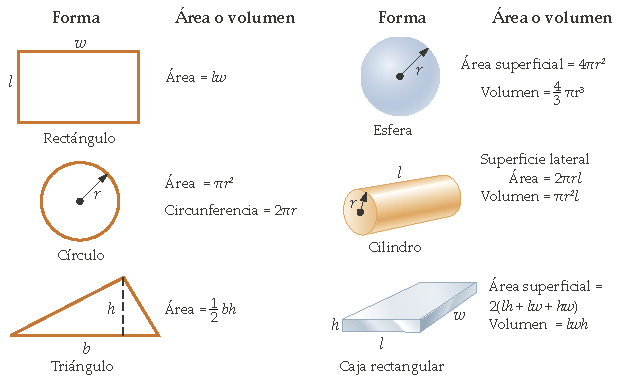
\includegraphics[width=0.90\linewidth]{figures/figuras_geo.pdf}
        \label{fig:append01}
    \end{figure}
\end{frame}
